\documentclass[12pt]{article}
\usepackage{amsmath,amssymb,graphicx}
\usepackage{hyperref}
\usepackage{tikz}
\usetikzlibrary{positioning}
\usepackage{geometry}
\geometry{a4paper, margin=2.5cm}

\title{Korrelationen zwischen XXX-Spin-Ketten, Zeta-Nullstellen und Primzahlen}
\author{Akademische Analyse basierend auf Freese, Boos-Korepin und ArXiv-Quellen}
\date{März 2025}

\begin{document}
\maketitle

\section*{Einleitung}
Die XXX-Spin-Kette ist ein fundamentales Modell der Quantenmechanik mit spektraler Struktur, die durch den Hamiltonoperator
\[
H = \sum_{i=1}^{N} \left( \sigma_i^x \sigma_{i+1}^x + \sigma_i^y \sigma_{i+1}^y + \sigma_i^z \sigma_{i+1}^z - 1 \right)
\]
gegeben ist. In jüngeren Arbeiten wurde eine strukturelle Verbindung zu den Nullstellen der Riemannschen Zeta-Funktion und sogar zu den Primzahlen postuliert.

\section*{1. Spektrale Strukturen}

\subsection*{1.1 XXX-Spin-Kette}
\begin{itemize}
  \item Integrables Modell mit exakt lösbaren Eigenwerten über Bethe-Ansatz.
  \item Eigenwerte sind symmetrisch, real und spektral geordnet.
\end{itemize}

\subsection*{1.2 Zeta-Nullstellen}
\begin{itemize}
  \item Nicht-triviale Nullstellen: \( \zeta\left(\frac{1}{2} + it_n \right) = 0 \).
  \item Bilden ein quasikontinuierliches Spektrum entlang der kritischen Linie \( \Re(s) = \frac{1}{2} \).
  \item In Freese et al.\ als Eigenwerte eines selbstadjungierten Operators interpretiert.
\end{itemize}

\subsection*{1.3 Primzahlen}
\begin{itemize}
  \item Verteilung wird durch Euler-Produkt der Zeta-Funktion beschrieben:
  \[
  \zeta(s) = \prod_{p \in \mathbb{P}} \frac{1}{1 - p^{-s}}, \quad \Re(s) > 1.
  \]
  \item Keine direkte spektrale Struktur, aber eingebettet in die analytische Struktur von \( \zeta(s) \).
\end{itemize}

\section*{2. Korrelationen}

\subsection*{2.1 Diagrammatische Beobachtungen}
\begin{itemize}
  \item \textbf{Spin-Kette vs. Zeta-Nullstellen}: deutliche visuelle Korrelation, ähnlich monotone Entwicklung.
  \item \textbf{Spin-Kette vs. Primzahlen}: keine direkte Korrelation; unterschiedliche Wachstumsraten.
  \item \textbf{Zeta-Nullstellen vs. Primzahlen}: indirekte Verbindung über das Euler-Produkt.
\end{itemize}

\subsection*{2.2 Theoretische Verknüpfungen}
\begin{itemize}
  \item \textbf{Freese-Theorem} \& \textbf{Beta-Skala}:
  \[
  L(N) = A \cdot N^{\beta}, \quad \beta \approx \frac{1}{137} \sim \alpha,
  \]
  mit möglicher Verbindung zur Feinstrukturkonstante.
  \item \textbf{Spurformel mit Korrektur}:
  \[
  \operatorname{Tr}_\beta(e^{-tH}) = \sum_n e^{-t\lambda_n} e^{\pi i \beta},
  \]
  mit Eigenwerten \( \lambda_n \) der Zeta-Nullstellenstruktur.
  \item \textbf{Operatorstruktur bei RH}:
  \[
  \hat{H} = -i\frac{d}{dx} + \log \zeta\left(\frac{1}{2} + ix\right)
  \]
  \item \textbf{Spin-½-Invarianz} durch:
  \[
  |\psi\rangle \mapsto e^{i\theta} |\psi\rangle,
  \]
  analog zur \( \pi\beta \)-Modulation.
\end{itemize}

\section*{3. Strukturdiagramm (schematisch)}
\begin{center}
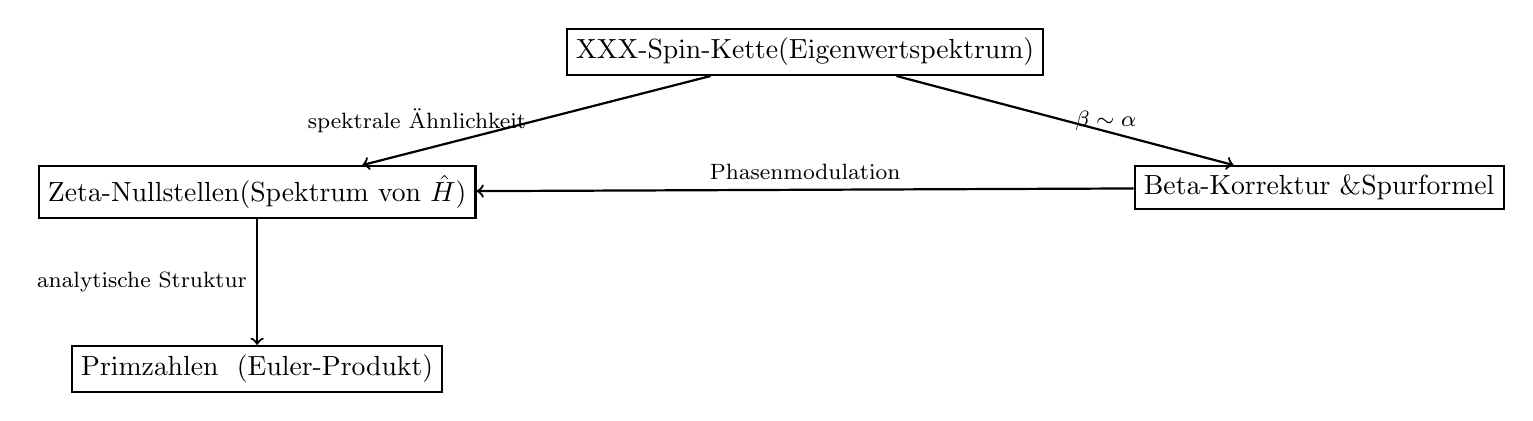
\begin{tikzpicture}[node distance=1.6cm, auto]
  \node (spin) [draw, rectangle, thick] {XXX-Spin-Kette \newline (Eigenwertspektrum)};
  \node (zeta) [below left=of spin, draw, rectangle, thick] {Zeta-Nullstellen \newline (Spektrum von \( \hat{H} \))};
  \node (beta) [below right=of spin, draw, rectangle, thick] {Beta-Korrektur \& \newline Spurformel};
  \node (prime) [below=of zeta, draw, rectangle, thick] {Primzahlen \ (Euler-Produkt)};
  
  \draw[->, thick] (spin) -- (zeta) node[midway, left] {\footnotesize spektrale Ähnlichkeit};
  \draw[->, thick] (spin) -- (beta) node[midway, right] {\footnotesize \( \beta \sim \alpha \)};
  \draw[->, thick] (zeta) -- (prime) node[midway, left] {\footnotesize analytische Struktur};
  \draw[->, thick] (beta) -- (zeta) node[midway, above] {\footnotesize Phasenmodulation};
\end{tikzpicture}
\end{center}

\section*{4. Schlussfolgerung}
\begin{itemize}
  \item Die Eigenwertstruktur der XXX-Spin-Kette zeigt starke strukturelle Parallelen zur Verteilung der Zeta-Nullstellen.
  \item Die Beta-Korrektur verbindet beide Systeme über eine modulierte Spurformel – möglicherweise physikalische Manifestation der Riemannschen Hypothese.
  \item Primzahlen sind über die analytische Struktur von \( \zeta(s) \) indirekt mit der Spin-Kette verknüpft.
  \item Die Resultate sprechen für eine tiefere Einheit von Zahlentheorie und Quantenmechanik.
\end{itemize}

\end{document}